
\section{Supplementary material for Chapter 3} \label{app:chapter3}

\vspace*{1cm}

% \subsection{PHENOFIT processes and parameters}

% \begin{figure}[htpb]
% \centering
% 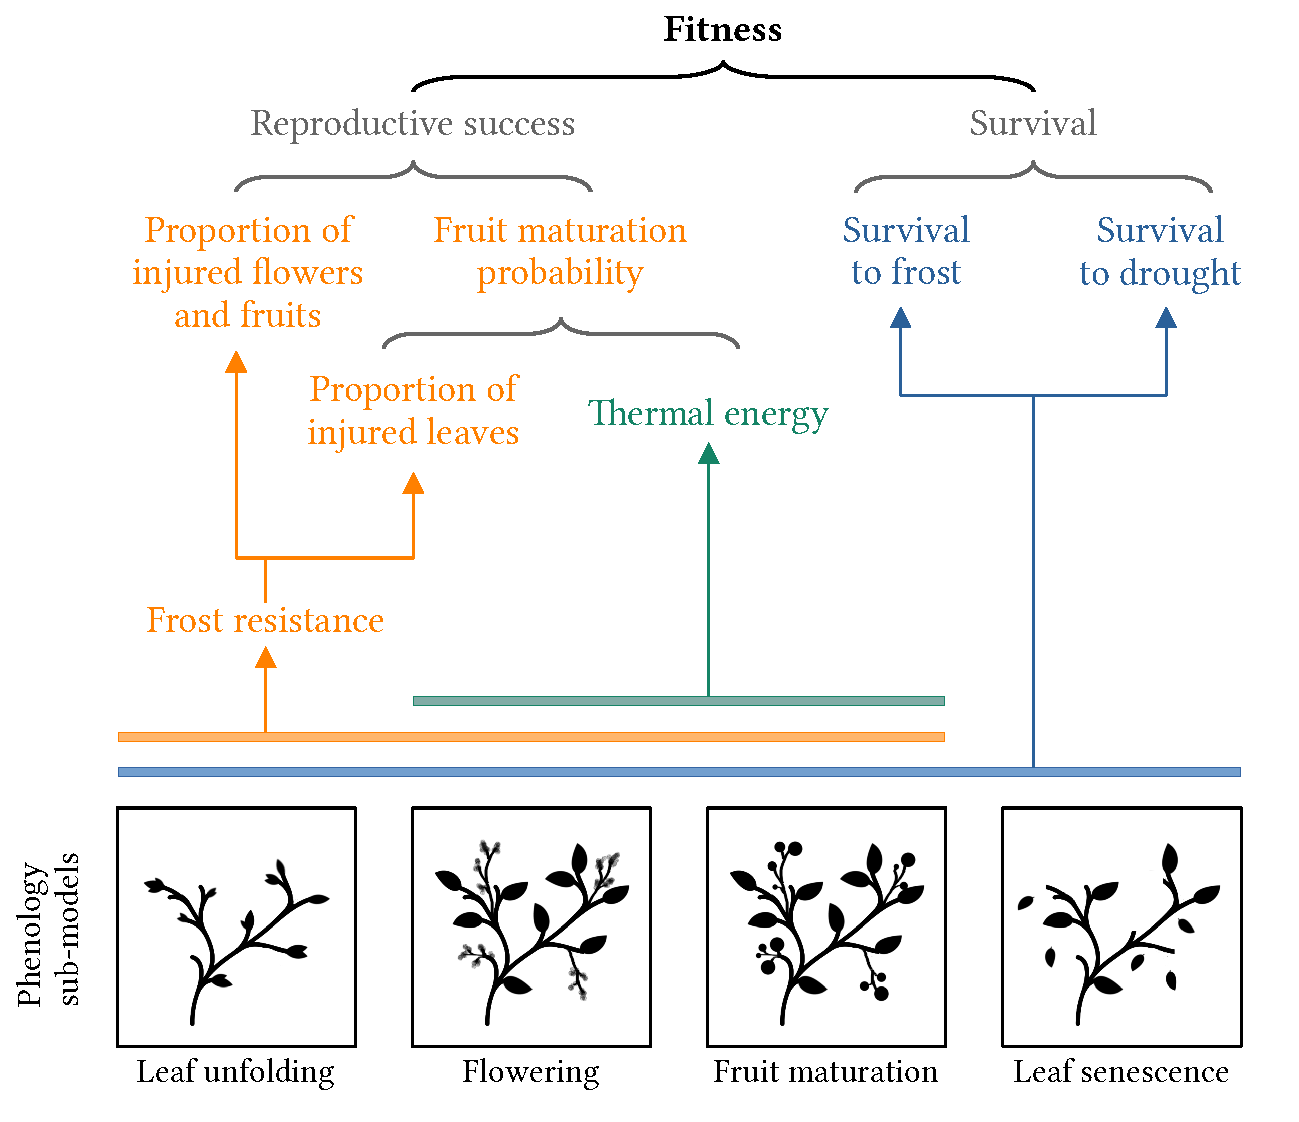
\includegraphics[width=0.9\textwidth]{phenofit.pdf}
% \caption{\textbf{}}
% \end{figure}

\newgeometry{left=1in,right=1in,top=0in,bottom=0.2in,nohead}
\begin{landscape}
\begin{table}[!h]
\fontsize{11}{10}\selectfont
\vspace*{-6em}
\caption{\bf{Description of PHENOFIT parameters for \emph{Fagus sylvatica}.}}
\begin{tabular}{ ccccc }

\hline
Process & Subprocess & Function & Parameter & Definition \\
\hline

\multirow{6}{5em}{Leaf unfolding} & \multirow{3}{7em}{Endodormancy} & \multirow{3}{7em}{Threshold inferior} 
& $t_0$ & Starting date of the endodormancy phase \\ 
& & & $T_b$ & Threshold temperature \\
& & & $C_{crit}$ & Critical state of development corresponding to dormancy break \\
\cmidrule{4-5}
& \multirow{3}{7em}{Ecodormancy} & \multirow{3}{7em}{Sigmoid} 
& $d_T$ & Slope at the inflection point \\ 
& & & $T_{50}$  & Mid-responsee temperature \\ 
& & & $F^{leaf}_{crit}$  & Critical state of development corresponding to leaf unfolding \\ 

\cmidrule{1-5}
\multirow{6}{5em}{Flowering} & \multirow{3}{7em}{Endodormancy} & \multirow{3}{7em}{Threshold inferior}
& $t_0$ &  Starting date of the endodormancy phase \\ 
& & & $T_b$ & Threshold temperature \\
& & & $C_{crit}$ & Critical state of development corresponding to dormancy break \\
\cmidrule{4-5}
& \multirow{3}{7em}{Ecodormancy} & \multirow{3}{7em}{Sigmoid} 
& $d_T$ & Slope at the inflection point \\ 
& & & $T_{50}$ & Mid-responsee temperature \\ 
& & & $F^{flower}_{crit}$ & Critical state of development corresponding to flowering \\ 

\cmidrule{1-5}
\multirow{6}{5em}{Fruit maturation} & \multirow{3}{7em}{Cell multiplication and growth} & \multirow{3}{7em}{Sigmoid} 
& aa & definition aa (sigmoid) \\ 
& & & bb & definition bb (sigmoid) \\
& & & $F^{fruit}_{crit}$ & Accumulation threshold above which accumulation starts \\
\cmidrule{4-5}
& \multirow{4}{7em}{Photosynthetic assimilate accumulation} & \multirow{4}{7em}{\citet{Wang1998}} 
& $T_{opt}$ & Optimal temperature \\ 
& & & $Mat_{moy}$  & Accumulation threshold above which maturation occurs \\ 
& & & $\sigma$  & Standard deviation \\ 
& & & ${pfe}_{50}$  & Prop. of injured leaves reducing by 50\% the flux of photosynthetic assimilates \\ 

\cmidrule{1-5}
{\multirow{6}{*}{Leaf senescence}} & & \multirow{6}{7em}{\citet{Delpierre2009}}
& $P_b$ & Photoperiod threshold below which photothermal accumulation starts \\ 
& & & $T_b$ & Max. temperature above which there no photothermal accumulation \\
& & & $\alpha$ & Effect of temperature on photothermal accumulation $\alpha$ \\
& & & $\beta$ & Effect of photoperiod on photothermal accumulation $\beta$ \\ 
& & & $S_{crit}$  & Accumulation threshold above which senescence occurs \\ 
& & & $\sigma^{senes}$  & Standard deviation \\ 

\cmidrule{1-5}
\multirow{10}{5em}{Frost hardening} & \multirow{2}{7em}{Leaf bud} & \multirow{8}{*}{\citet{Leinonen1996}}
& $FH^{leaf}_{min}$ & Minimum level of frost hardiness \\ 
& & & $FHT^{leaf}_{max}$/$FHP^{leaf}_{max}$ & Maximum level of the increase of frost hardiness induced by temperature/photoperiod \\
\cmidrule{4-5}
& \multirow{2}{7em}{Flower bud} &
& $FH^{flower}_{min}$ & Minimum level of frost hardiness \\ 
&  & & $FHT^{flower}_{max}$, $FHP^{flower}_{max}$ & Maximum level of the increase of frost hardiness induced by temperature/photoperiod \\
\cmidrule{4-5}
& \multirow{2}{7em}{Thermal control} &
& $Te_1$ & Upper limit of the effective range of temperature \\ 
& & & $Te_2$  & Lower limit of the effective range of temperature\\ 
\cmidrule{4-5}
& \multirow{2}{7em}{Photoperiod control} &
& $NL_1$ & Lower limit of the effective range of photoperiod \\ 
& & & $NL_2$  & Upper limit of the effective range of photoperiod\\ 
\cmidrule{4-5}
& \multirow{2}{7em}{Fruit} & \multirow{2}{*}{Piecewise linear}
& FHfrmax1 & Minimum level of frost hardiness \\ 
& & & FHfrmax2 & Maximum level of frost hardiness \\

\cmidrule{1-5}
\multirow{4}{5em}{Water stress} & \multicolumn{2}{c}{\multirow{4}{*}{Precipitation range}}
& $pp_{extlow}$ & $1^{th}$ percentile \\
\multicolumn{3}{c}{} & $pp_{low}$ & $5^{th}$ percentile \\
\multicolumn{3}{c}{} & $pp_{high}$ & $95^{th}$ percentile \\
\multicolumn{3}{c}{} & $pp_{exthigh}$ & $99^{th}$ percentile \\ 
\hline

\end{tabular}
\vspace*{-4em}
\end{table}
\end{landscape}
\restoregeometry

\newpage

%\rotatebox{90}{
%\begin{minipage}{\textheight}
%\begin{table}[!h]
\fontsize{11}{10}\selectfont
\vspace*{-6em}
\caption{\bf{Description of PHENOFIT parameters for \emph{Fagus sylvatica}.}}
\begin{tabular}{ ccccc }

\hline
Process & Subprocess & Function & Parameter & Definition \\
\hline

\multirow{6}{5em}{Leaf unfolding} & \multirow{3}{7em}{Endodormancy} & \multirow{3}{7em}{Threshold inferior} 
& $t_0$ & Starting date of the endodormancy phase \\ 
& & & $T_b$ & Threshold temperature \\
& & & $C_{crit}$ & Critical state of development corresponding to dormancy break \\
\cmidrule{4-5}
& \multirow{3}{7em}{Ecodormancy} & \multirow{3}{7em}{Sigmoid} 
& $d_T$ & Slope at the inflection point \\ 
& & & $T_{50}$  & Mid-responsee temperature \\ 
& & & $F^{leaf}_{crit}$  & Critical state of development corresponding to leaf unfolding \\ 

\cmidrule{1-5}
\multirow{6}{5em}{Flowering} & \multirow{3}{7em}{Endodormancy} & \multirow{3}{7em}{Threshold inferior}
& $t_0$ &  Starting date of the endodormancy phase \\ 
& & & $T_b$ & Threshold temperature \\
& & & $C_{crit}$ & Critical state of development corresponding to dormancy break \\
\cmidrule{4-5}
& \multirow{3}{7em}{Ecodormancy} & \multirow{3}{7em}{Sigmoid} 
& $d_T$ & Slope at the inflection point \\ 
& & & $T_{50}$ & Mid-responsee temperature \\ 
& & & $F^{flower}_{crit}$ & Critical state of development corresponding to flowering \\ 

\cmidrule{1-5}
\multirow{6}{5em}{Fruit maturation} & \multirow{3}{7em}{Cell multiplication and growth} & \multirow{3}{7em}{Sigmoid} 
& aa & definition aa (sigmoid) \\ 
& & & bb & definition bb (sigmoid) \\
& & & $F^{fruit}_{crit}$ & Accumulation threshold above which accumulation starts \\
\cmidrule{4-5}
& \multirow{4}{7em}{Photosynthetic assimilate accumulation} & \multirow{4}{7em}{\citet{Wang1998}} 
& $T_{opt}$ & Optimal temperature \\ 
& & & $Mat_{moy}$  & Accumulation threshold above which maturation occurs \\ 
& & & $\sigma$  & Standard deviation \\ 
& & & ${pfe}_{50}$  & Prop. of injured leaves reducing by 50\% the flux of photosynthetic assimilates \\ 

\cmidrule{1-5}
{\multirow{6}{*}{Leaf senescence}} & & \multirow{6}{7em}{\citet{Delpierre2009}}
& $P_b$ & Photoperiod threshold below which photothermal accumulation starts \\ 
& & & $T_b$ & Max. temperature above which there no photothermal accumulation \\
& & & $\alpha$ & Effect of temperature on photothermal accumulation $\alpha$ \\
& & & $\beta$ & Effect of photoperiod on photothermal accumulation $\beta$ \\ 
& & & $S_{crit}$  & Accumulation threshold above which senescence occurs \\ 
& & & $\sigma^{senes}$  & Standard deviation \\ 

\cmidrule{1-5}
\multirow{10}{5em}{Frost hardening} & \multirow{2}{7em}{Leaf bud} & \multirow{8}{*}{\citet{Leinonen1996}}
& $FH^{leaf}_{min}$ & Minimum level of frost hardiness \\ 
& & & $FHT^{leaf}_{max}$/$FHP^{leaf}_{max}$ & Maximum level of the increase of frost hardiness induced by temperature/photoperiod \\
\cmidrule{4-5}
& \multirow{2}{7em}{Flower bud} &
& $FH^{flower}_{min}$ & Minimum level of frost hardiness \\ 
&  & & $FHT^{flower}_{max}$, $FHP^{flower}_{max}$ & Maximum level of the increase of frost hardiness induced by temperature/photoperiod \\
\cmidrule{4-5}
& \multirow{2}{7em}{Thermal control} &
& $Te_1$ & Upper limit of the effective range of temperature \\ 
& & & $Te_2$  & Lower limit of the effective range of temperature\\ 
\cmidrule{4-5}
& \multirow{2}{7em}{Photoperiod control} &
& $NL_1$ & Lower limit of the effective range of photoperiod \\ 
& & & $NL_2$  & Upper limit of the effective range of photoperiod\\ 
\cmidrule{4-5}
& \multirow{2}{7em}{Fruit} & \multirow{2}{*}{Piecewise linear}
& FHfrmax1 & Minimum level of frost hardiness \\ 
& & & FHfrmax2 & Maximum level of frost hardiness \\

\cmidrule{1-5}
\multirow{4}{5em}{Water stress} & \multicolumn{2}{c}{\multirow{4}{*}{Precipitation range}}
& $pp_{extlow}$ & $1^{th}$ percentile \\
\multicolumn{3}{c}{} & $pp_{low}$ & $5^{th}$ percentile \\
\multicolumn{3}{c}{} & $pp_{high}$ & $95^{th}$ percentile \\
\multicolumn{3}{c}{} & $pp_{exthigh}$ & $99^{th}$ percentile \\ 
\hline

\end{tabular}
\vspace*{-4em}
\end{table}
%\end{minipage}}

\subsection{Leinonen frost hardiness model}

The model developed by \cite{Leinonen1996} predicts the frost hardiness of tree buds, i.e. their ability to withstand frost without being damaged. The model uses daily temperature, photoperiod, and bud development state (phenological state) as the drivers of bud hardening and dehardening. In particular, a tree undergoes acclimation in response to two factors : decreasing temperatures and shorter days. The damage caused by freezing thus depends on the minimum temperature of day $t$ and the actual frost hardiness $FH_t$ reach on day $t$:
\begin{equation}
FH_t = FH_{min} + CR_t * (\Delta FHT_t + \Delta FHP_t)
\end{equation}

\noindent $FH_{min}$ is the minimum level of frost hardening of a bud expressed in degree celsius and it correspond to the level after bud break when leaves have just unfold (see table above), $CR_t$ is the hardening competence (which depends on the phenological state), $\Delta FHT_t$ is the increase of frost hardiness induced by temperature and $\Delta FHP_t$ is the increase of frost hardiness induced by photoperiod.

\paragraph{Exposure to cold temperatures}

The temperature component $\Delta FHT_t$ is modelled by a piece-wise linear function depending on the daily minimum temperature $T_t$:

\begin{equation}
  \Delta FHT_t =
    \begin{cases}
      FHT_{max} & \text{if $T_t < Te_2$}\\
      FHT_{max}*(1-\frac{T_t-Te_2}{Te_1-Te_2}) & \text{if $Te_2 \leq T_t \leq Te_1$}\\
      0 & \text{if $T_t > Te_1$}
    \end{cases}       
\end{equation}

\noindent $FHT_{max}$, $Te_2$, and $Te_1$ are described in the table above. $FHT_{max}$ correspond to the maximum level of frost hardiness that temperature can induce when the bud is fully dormant during winter.

\paragraph{Photoperiod sensitivity}

The photoperiod component $\Delta FHP_t$ is modelled by a piece-wise linear function depending on the daily night length $NL_t$:

\begin{equation}
  \Delta FHP_t =
    \begin{cases}
      FHP_{max} & \text{if $NL_t > NL_2$}\\
      FHP_{max}*\frac{NL_t-NL_1}{NL_2-NL_1} & \text{if $NL_1 \leq NL_t \leq NL_2$}\\
      0 & \text{if $NL_t < NL_1$}
    \end{cases}       
\end{equation}

\noindent $FHP_{max}$, $NL_2$, and $NL_1$ are described in the table above. $FHP_{max}$ correspond to the maximum level of frost hardiness that photoperiod can induce when the bud is fully dormant during winter. $FHT_{max}$ + $FHP_{max}$ corresponds to the maximum level of frost hardiness that the bud can reach when it is fully dormant during winter. 

\newpage

\subsection{Fitted parameter values of beech}

\begin{figure}[hp]
\vspace*{-0.5cm}
\centering
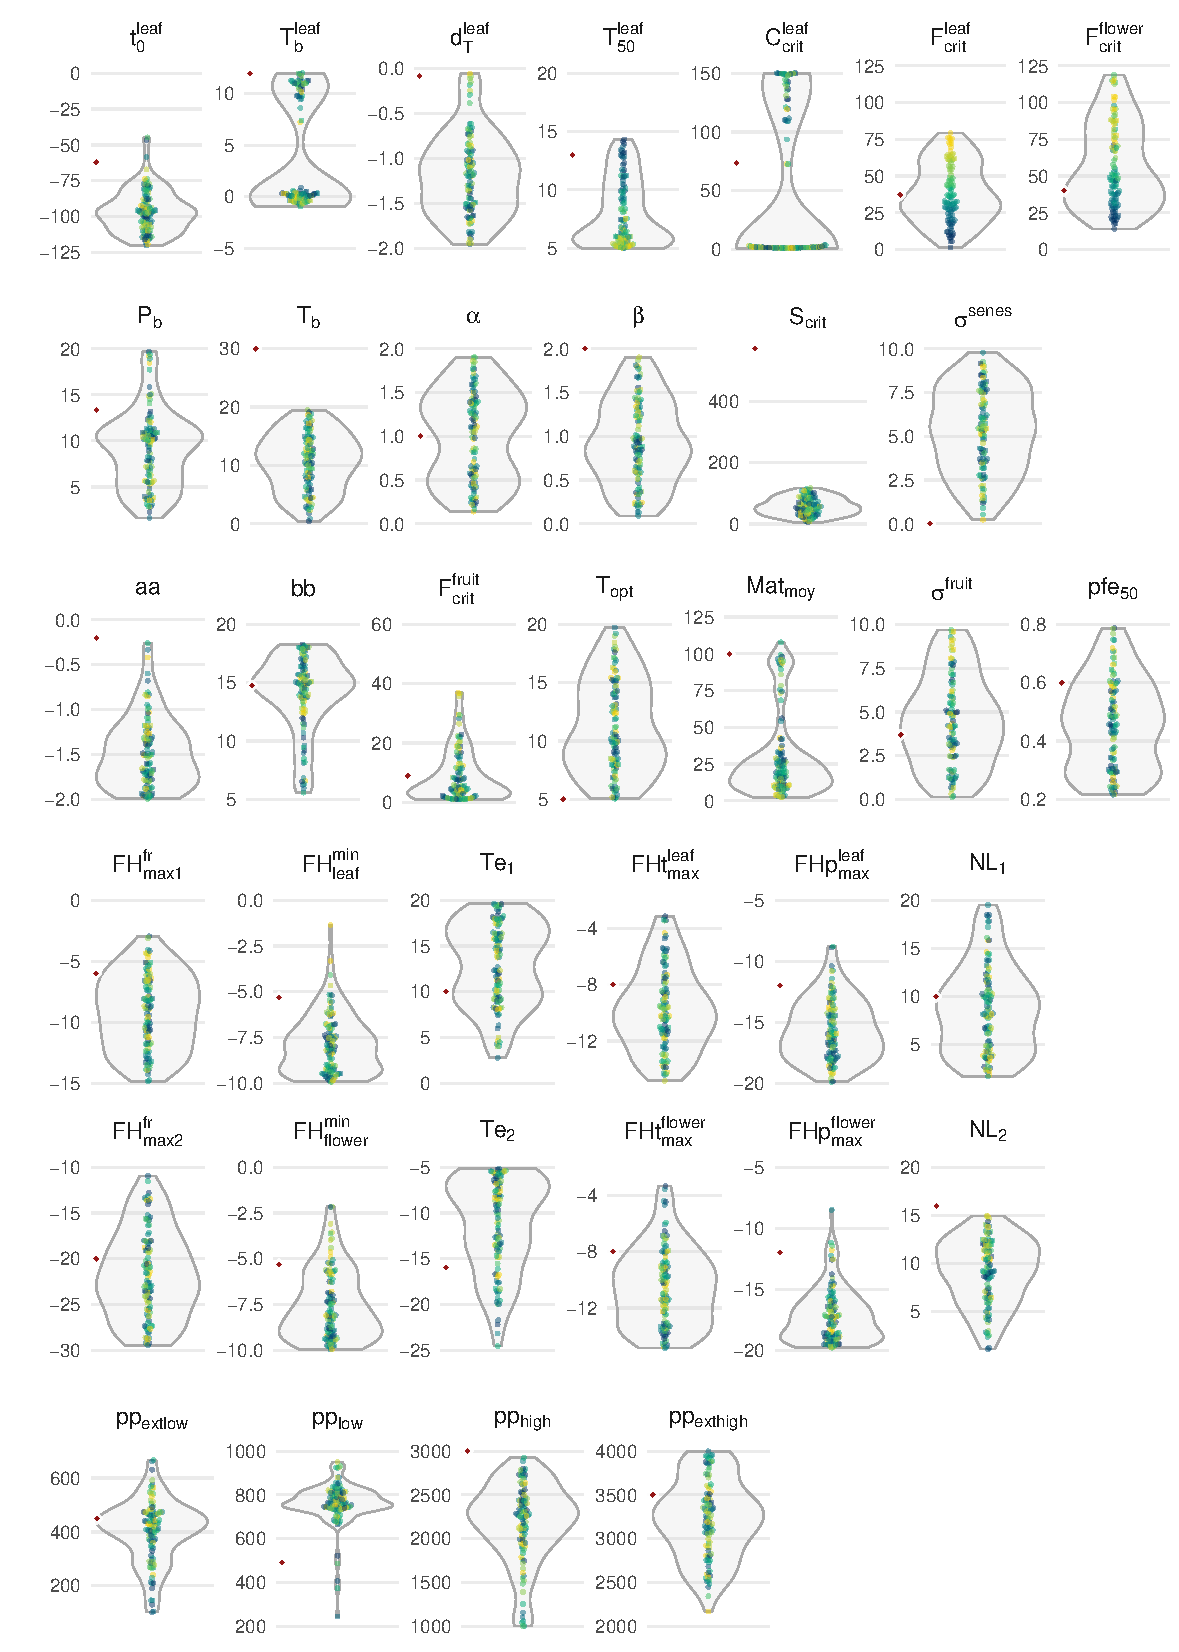
\includegraphics[width=1\textwidth]{chapter3/figs/parameters_fsylvatica.pdf}
\caption{\textbf{CMA-ES calibration of PHENOFIT parameters for beech.} Each panel is a parameter. Y-axis limits are lower and upper bounds used during calibration. Each point is a calibrated parameter value, colour gradient is based on $F_{crit}^{leaf}$ values. Red diamonds are parameter values obtained with expert calibration.}
\vspace*{-5cm}
\end{figure}

\newpage

\subsection{Phenological records in Europe}

\begin{figure}[hp]
\vspace*{-0.3cm}
\centering
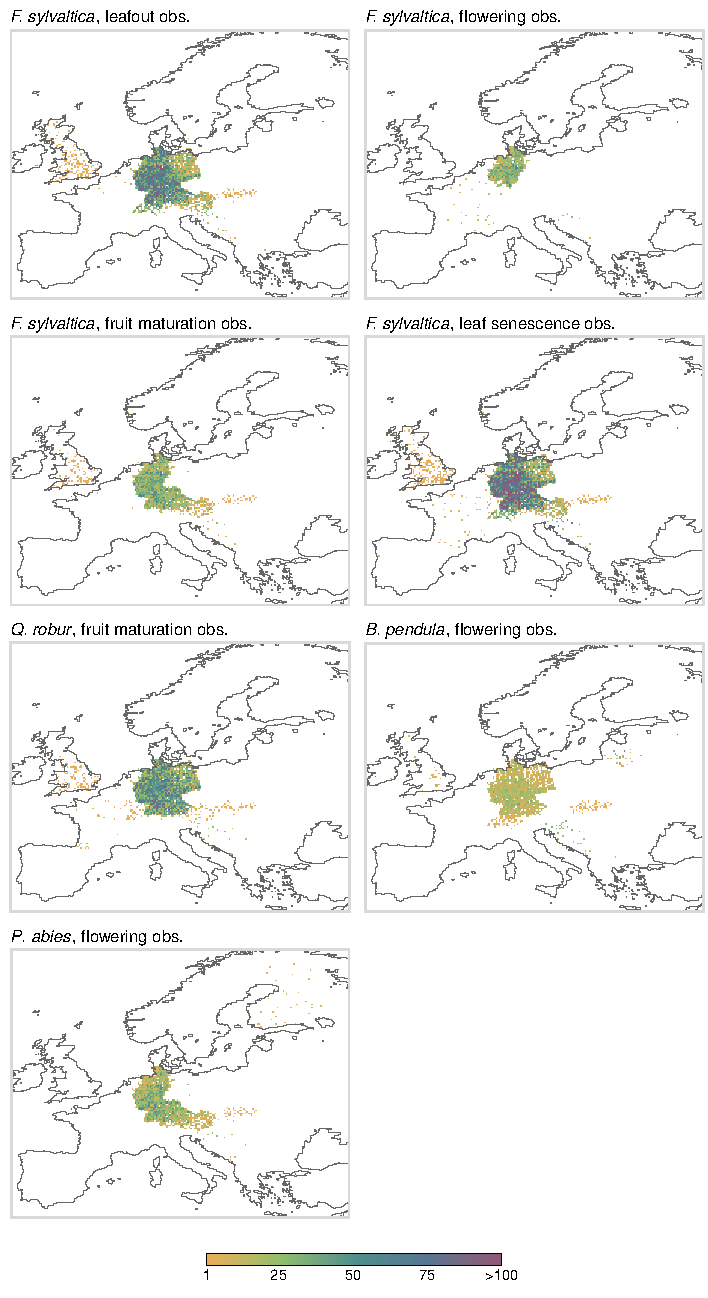
\includegraphics{chapter3/figs/figS1-1.pdf}
\caption{\textbf{Observations used to calculate RMSE on simulated phenological dates.} These observations were extracted from the PEP725 (\url{pep725.eu}) and the TEMPO (\url{data.pheno.fr}) databases, for the period 1970-2000. Note that they were aggregated to 0.2\degree~spatial resolution, to enhance the readability of the figure.}
\label{fig:phenologicalrecords}
\vspace*{-5cm}
\end{figure}

\clearpage

\subsection{Climatic dissimilarity over the Holocene}

\begin{figure}[htpb]
\centering
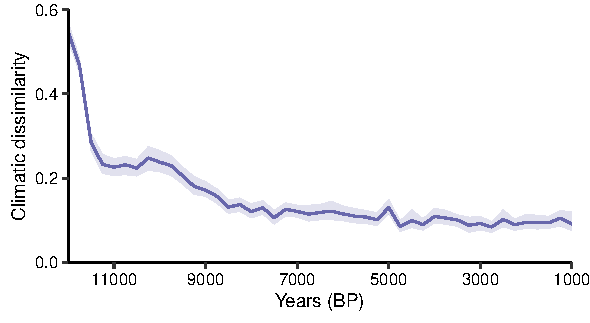
\includegraphics{chapter3/figs/figS2-1.pdf}
\caption{\textbf{Climatic dissimilarity between past conditions and historical conditions.} The metric was calculated as the Sørensen dissimilarity between climatic hypervolumes (a metric of overlap in multidimensional space). See \cite{VanderMeersch2024} for details.}
\label{fig:dissimilarity}
\end{figure}